\chapter{Deep Feedforward Networks 2}

\section{Networks}%
\label{sec:label}

We can connect ``neurons'', such that the output of one neuron becomes the input to another neuron. Let's think about this in a more structured way. Usually, we have more than one node (neuron). We usually arrange those in ``layers''. Thus, we have a ``beginning layer'', which takes no input from other neurons. However, those neurons give their output to neurons in layer 2. This continues until you reach the ending layer.

Remember, that we can assign to each neuron a \textit{weight}, such that it bears more or less power, or even negative power (for example, we would want something negative to be negatively rewarded). Other than this, we also have an activation function, which we ignore for now.

\begin{figure}[ht]
	\centering
	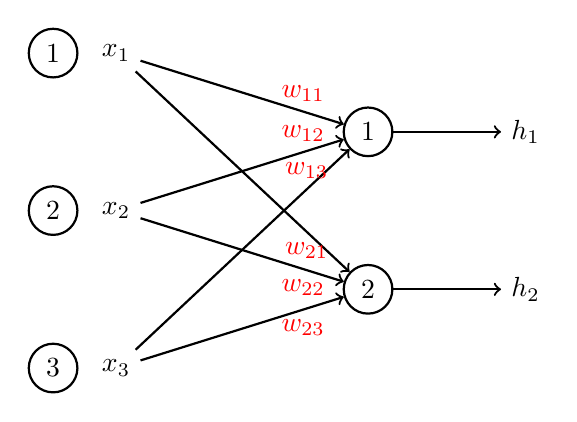
\begin{tikzpicture}[node distance={30mm}, thick, main/.style = {draw, circle}]

		\node[main] (1) at (0,0) {1};
		\node[main] (2) at (0,-2) {2};
		\node[main] (3) at (0,-4) {3};
		\node[] (x1) at (0.8,0) {$x_{1}$};
		\node[] (x2) at (0.8,-2) {$x_{2}$};
		\node[] (x3) at (0.8,-4) {$x_{3}$};

		\node[main] (1r) at (4,-1) {1};
		\node[main] (2r) at (4,-3) {2};
		\node[] (h1) at (6,-1) {$h_{1}$};
		\node[] (h2) at (6,-3) {$h_{2}$};

		\draw[->] (x1) -- node[pos=0.8, above, text=red] {$w_{11}$} (1r);
		\draw[->] (x2) -- node[pos=0.8, above, text=red] {$w_{12}$} (1r);
		\draw[->] (x3) -- node[pos=0.8, above, text=red] {$w_{13}$} (1r);
		\draw[->] (x1) -- node[pos=0.8, below, text=red] {$w_{21}$} (2r);
		\draw[->] (x2) -- node[pos=0.8, below, text=red] {$w_{22}$} (2r);
		\draw[->] (x3) -- node[pos=0.8, below, text=red] {$w_{23}$} (2r);

		\draw[->] (1r) -- (h1);
		\draw[->] (2r) -- (h2);
	\end{tikzpicture}
	\caption{\label{fig:network} A Network.}
\end{figure}

In Figure~\ref{fig:network} we see an example of such a ``network''. For the node $1$ we get $h_{1} = w_{11} \cdot x_{1} + w_{12} \cdot x_{2} + w_{13} \cdot x_{3}$. For the node $2$ we get $h_{2} = w_{21} \cdot x_{1} + w_{22} \cdot x_{2} +  w_{23} \cdot x_{3}$. From Section~\ref{sec:systemoflinearequations} we know that we can rewrite this as:

\begin{equation*}
	\begin{pmatrix}
		h_{1} \\
		h_{2}
	\end{pmatrix} =
	\begin{pmatrix}
		w_{11} & w_{12} & w_{13} \\
		w_{21} & w_{22} & w_{23}
	\end{pmatrix} \cdot \begin{pmatrix}
		x_{1} \\
		x_{2} \\
		x_{3}
	\end{pmatrix}
\end{equation*}

We can add a \textit{bias} to this (which allows for us to set the threshold to be $>0$ rather than $> \text{threshold}$. This is also trainable.):
\begin{equation*}
	\begin{pmatrix}
		h_{1} \\
		h_{2}
	\end{pmatrix} =
	\begin{pmatrix}
		w_{11} & w_{12} & w_{13} & {\color{red} b_{1}} \\
		w_{21} & w_{22} & w_{23} & {\color{red} b_{2}}
	\end{pmatrix} \cdot \begin{pmatrix}
		x_{1} \\
		x_{2} \\
		x_{3} \\
		{\color{red} 1}
	\end{pmatrix}
\end{equation*}


\begin{figure}[ht]
	\centering
	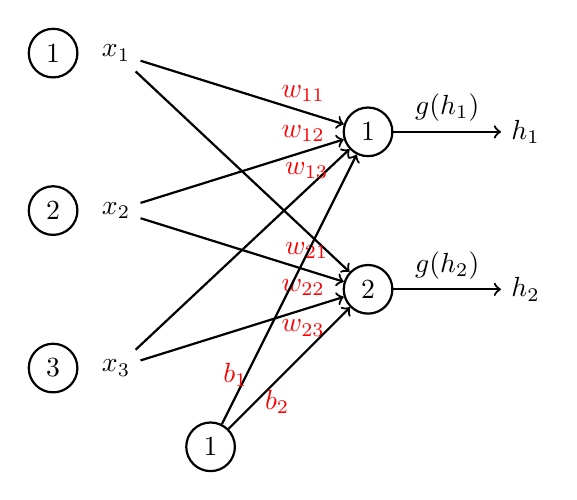
\begin{tikzpicture}[node distance={30mm}, thick, main/.style = {draw, circle}]

		\node[main] (1) at (0,0) {1};
		\node[main] (2) at (0,-2) {2};
		\node[main] (3) at (0,-4) {3};
		\node[] (x1) at (0.8,0) {$x_{1}$};
		\node[] (x2) at (0.8,-2) {$x_{2}$};
		\node[] (x3) at (0.8,-4) {$x_{3}$};

		\node[main] (b1) at (2, -5) {1};

		\node[main] (1r) at (4,-1) {1};
		\node[main] (2r) at (4,-3) {2};
		\node[] (h1) at (6,-1) {$h_{1}$};
		\node[] (h2) at (6,-3) {$h_{2}$};

		\draw[->] (x1) -- node[pos=0.8, above, text=red] {$w_{11}$} (1r);
		\draw[->] (x2) -- node[pos=0.8, above, text=red] {$w_{12}$} (1r);
		\draw[->] (x3) -- node[pos=0.8, above, text=red] {$w_{13}$} (1r);
		\draw[->] (x1) -- node[pos=0.8, below, text=red] {$w_{21}$} (2r);
		\draw[->] (x2) -- node[pos=0.8, below, text=red] {$w_{22}$} (2r);
		\draw[->] (x3) -- node[pos=0.8, below, text=red] {$w_{23}$} (2r);

		\draw[->] (1r) -- node[pos=0.5, above] {$g(h_{1})$} (h1);
		\draw[->] (2r) -- node[pos=0.5, above] {$g(h_{2})$} (h2);

		\draw[->] (b1) -- node [pos=0.1, above, text=red] {$b_{1}$} (1r);
		\draw[->] (b1) -- node [pos=0.4, below, text=red] {$b_{2}$} (2r);
	\end{tikzpicture}
	\caption{\label{fig:network_bias_activation} A Network with an activation function and bias.}
\end{figure}

In Figure~\ref{fig:network_bias_activation} you see a network which has a bias, and an activation function going from the neurons 1 and 2 to respectively $h_{1}$ and $h_{2}$. In this instance we call the activation functions $g(x)$. Thus, using the matrix format, we get
\[
	y = g(\mathbf{Wx}+b)
\]

We can summarize these networks to their essential parts. We receive the vector $\mathbf{x}$ and perform an \textit{affine transformation} according to the weight matrix $h' = Wx + b$. Afterwards, the internal representation is fed through an activation function $h_{i} = g(h_{i}')$, and generator the input vector $h$ for the next layer.

From now on we change our notation a bit. We define the following:
\begin{itemize}
	\item $x$ denotes the input.
	\item $W$ denotes the weight matrices. $w$ denotes the weight vectors.
	\item $h$ denotes the hidden layer ``outputs''.
	\item $y$ is the final output of the network.
\end{itemize}

You can think of a deeper network in terms of functions. Let $f^{(n)}$ be layer $n$. Then $f(x) = f^{(3)}(f^{(2)}(f^{1}(x)))$. We say the length of this chain is the \textit{depth} of the model. This is where the name \textit{deep learning} comes from. The final layer is the outermost in function terminology, in the case shown above it is $f^{(3)}$.

\section{Hidden Layers}%
\label{sec:label}

The behaviour of the ``hidden layers'' is not directly specified by the data. It is up to the learning algorithm to decide how to use those layers, such that the final output is close to $y$. The training data does not tell each individual layer what it should do. Rather, one of the main tasks of the algorithm is to define the appropriate structure of the network and hidden layers. The reason we call these layers ``hidden'', is that the desired output for these layers is not shown.

To represent non-linear functions of $x$ (that is, the input), we apply a linear model to the transformed input \(\phi(x)\) with  a non-linear \(\phi\). The function is non-linear with relation to \(\phi\), but not with relation to \(\phi(x)\). Thus, we can think of \(\phi\) as providing a set of features resulting in a new representation for $x$.

There are multiple ways to ``get'' \(\phi\):
\begin{enumerate}
	\item Generic functions: There exists a set of useful kernel functions.
	\item Manually engineer \(\phi\): Possible, but laborious and not transformable.
	\item With \textit{deep learning} we \textit{learn} \(\phi\).
\end{enumerate}

We'll use the XOR problem as a way to illustrate the importance of activation functions in neural networks. XOR is a logical function that takes two binary inputs (either 0 or 1) and outputs a 0 if both inputs are the same (either both 0 or both 1) and a 1 if the inputs are different.

The XOR problem is significant because it cannot be solved with a simple linear model: there is no linear function (i.e., no straight line or hyperplane) that can separate the two classes (output 0 vs. output 1) in a 2-dimensional space. This lack of linear separability shows that we need non-linear activation functions to model such problems successfully.

So, we are trying to \textit{approximate} the XOR function. Our training points are the following:
\[
	X = \left\{ [0,0]^{T}, [1,0]^{T}, [0,1]^{T}, [1,1]^{T} \right\}
\]

Let's use a Feedforward Network. We'll have one hidden layer, containing two units. These two units we  call $x_{1}$ and $x_{2}$. These are mapped to the hidden layer using the \textbf{weight matrix} $W$. This holds information about how much influence each input has on each hidden unit.

Next, the hidden layer outputs $h_{1}$ and $h_{2}$ are transformed into the final output $y$. We represent this step by a \textit{weight vector}, which we denote by $w$. This described how the hidden layer is mapped to the output. It contains the weights that determine how much each hidden unit $h_{1}$​ and $h_{2}$​ influences the output. Similar to the input-to-hidden transformation, this step involves another linear transformation, where we compute the dot product between the vector $w$ and the hidden layer activations to calculate the output $y$.

In this explanation, we are omitting bias terms, which would normally be added to the weighted sums before applying the activation function. Biases help shift the activation function and add more flexibility to the model, but for simplicity, they are not included here.


\begin{figure}[ht]
	\centering
	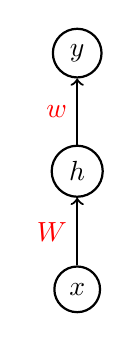
\begin{tikzpicture}[node distance={30mm}, thick, main/.style = {draw, circle}]

		\node[main] (1) at (0,0) {$y$};
		\node[main] (2) at (0,-1.5) {$h$};
		\node[main] (3) at (0,-3) {$x$};

		\draw[->] (3) -- node[pos=0.5, left, text=red] {$W$} (2);
		\draw[->] (2) -- node[pos=0.5, left, text=red] {$w$} (1);
	\end{tikzpicture}
	\caption{\label{fig:Simple-Network} A network with matrix $W$ and vector $w$.}
\end{figure}

In Figure~\ref{fig:Simple-Network} the first layer is the hidden layer, $h$. This is computed by the function $h = f^{(1)}(x; W, c)$ where $c$ are bias variables and $W$ is the matrix. The second layer, which is the output layer, $y$. This is computed by the function $y = f^{(2)}(h; w, b)$. Here $w$ are the weights in a vector format. The output is linear regression applied to $h$ rather than $x$. Thus, the complete model can be described in terms of functions like this:

\[
	f(x; W, c, w, b) = f^{(2)}(f^{(1)}(x; W, c), w, b)
\]

Now, if we choose both $f^{(1)}$ and $f^{(2)}$ to be linear, the total function will still be linear, which we have shown in this example to be insufficient. Therefore, we need an \textit{activation function}. Recall our function:
\[
	y = x^{T}w+b
\]
Typically, we choose an activation function to be applied element-wise: $h_{i} = g(x^{T}W_{:i}+c_{i})$. Now we define the activation function to be $g(z) = \max\{0,z\}$. This is called ReLU. This is already a non-linear transformation, although it is piecewise linear. This  has some nice properties which make gradient-based learning easy, and generalizes well.

Now, let's go back to our XOR problem. Our complete function is now:

\[
	f(x; W, c, w, b) = w^{T}\max \left\{ 0, W^{T}x+c \right\} + b
\]

Let us use the following weights:

\[
	W = \begin{bmatrix}
		1 & 1 \\
		1 & 1
	\end{bmatrix}, c = \begin{bmatrix}
		0 \\
		-1
	\end{bmatrix}, w = \begin{bmatrix}
		1 \\
		-2
	\end{bmatrix}, b = 0, X = \begin{bmatrix}
		0101 \\
		0011
	\end{bmatrix}^{T}
\]

Then we get the following transformations:
\begin{equation}
	XW = \begin{bmatrix}
		0 & 0 \\
		1 & 1 \\
		1 & 1 \\
		2 & 2
	\end{bmatrix}
\end{equation}
\begin{equation}
	XW + c = \begin{bmatrix}
		0 & -1 \\
		1 & 0  \\
		1 & 0  \\
		2 & 1
	\end{bmatrix}
\end{equation}
\begin{equation}
	\max \left\{ 0,XW+c \right\} = \begin{bmatrix}
		0 & 0 \\
		1 & 0 \\
		1 & 0 \\
		2 & 1
	\end{bmatrix}
\end{equation}
\begin{equation}
	\begin{bmatrix}
		0 & 0 \\
		1 & 0 \\
		1 & 0 \\
		2 & 1
	\end{bmatrix}w = \begin{bmatrix}
		0 \\
		1 \\
		1 \\
		0
	\end{bmatrix}
\end{equation}

This works for guessing XOR. However, we ``cheated'' doing this, as we already knew the weights. In reality there are millions of parameters, which we have to actually learn.

In general, for a hidden unit (that is, a neuron in a hidden layer) accepts a vector of inputs, which we denote $x$. Then it computes an affine transformation of these inputs: $h' = Wx+b$, where $W$ is the weight matrix and $b$ is the bias vector. After this transformation, a non-linear function (such as ReLU) $g(h')$ is applied element-wise to the result. However, the main difference between the hidden units, are the types of activation functions they use.

We now turn our attention to which activation functions to choose. It's an active research area, to design these. Usually ReLU is an excellent ``default'' choice, however, there are many other available. Usually, we find out which we want to use through trial-and-error, as there is no ``one-size-fits-all'' approach.

For ReLU it's good practice to set all elements of $b$ to a small value, such as $0.1$. This makes it likely that ReLU will be initially active for most training samples and allow derivatives to pass through. However, for ReLU it cannot learn from examples whose activation is zero. We'll look at three generalizations of ReLU, all based on using a non-zero slope $\alpha_{i}$ when $z_{i} < 0$:
\begin{equation*}
	h_{i} = g(z,\alpha)_{i} = \max{0,z_{i}} + \alpha_{i}\min(0,z_{i})
\end{equation*}
\begin{itemize}
	\item \textbf{Absolute-value rectification:}
	      \begin{itemize}
		      \item Fixes $\alpha_{i} = -1$ to obtain $g(z) = |z|$
	      \end{itemize}

	\item \textbf{Leaky ReLU}:
	      \begin{itemize}
		      \item Fixes \(\alpha_{i}\) to a small value like 0.01
	      \end{itemize}
	\item \textbf{Parametric ReLU or PReLU}
	      \begin{itemize}
		      \item Treats \(\alpha_{i}\) as a learnable parameter
	      \end{itemize}
\end{itemize}

Before using ReLU, most neural networks used logistic sigmoid \(g(z) = \sigma(z)\), or $g(z) = \text{tanh}(z)$. These are closely related, because $\text{tanh}(z) = 2\sigma(2z)-1$. Sigmoid units are used to predict probability that a binary variable is 1.

Following are examples of some other activation functions:
\begin{itemize}
	\item Cosine: $h = \cos(Wx+b)$
	      \begin{itemize}
		      \item Feedforward networks on MNIST obtained error rate of less than 1%
	      \end{itemize}
	\item Radial Basis
	      \begin{itemize}
		      \item $h_{i} = exp(- \frac{1}{\sigma^{2}} \left| \left| W_{:j}-x \right| \right|^{2})$
		      \item This becomes more active as $x$ approaches a template $W_{:,i}$
	      \end{itemize}
	\item Softplus
	      \begin{itemize}
		      \item $g(a) = \zeta(a) = log(1+e^{a})$
		      \item Smooth version of the rectifier
	      \end{itemize}
	\item Hard tanh
	      \begin{itemize}
		      \item $g(a) = \max\{-1, \min(1,a)\}$
		      \item Shaped similar to tanh and the rectifier but it is bounded
	      \end{itemize}
\end{itemize}

\section{Output Units}%
\label{sec:label}

The choice of a cost function is \textbf{tightly} coupled with the choice of output unit. Most of the time we use cross-entropy between data distribution and model distribution. The choice of how to represent the output then determines the form of the cross-entropy function.

Any output unit is, in principle, also usable as a hidden unit. A feedforward network provides a hidden set of features:
\[
	h = f(x;\theta)
\]

The role of the output layer is to provide some additional transformation from the features to the task that
network must perform. Following are some of the most common output units:
\begin{itemize}
	\item \textbf{Linear Units}: Used for regressions, no non-linearity.
	\item \textbf{Sigmoid Units}: used for binary classification.
	\item \textbf{Softmax Units}: used for general classification.
\end{itemize}

A linear unit is a simple output which is based on affine transformation with no non-linearity. Given features $h$, a layer of linear output units produce a vector:
\[
	\hat{y} = W^{T}h + b
\]

Sigmoid units are used for the task of predicting value of a binary variable.

Sigmoid units always give a gradient $\hat{y} = \sigma(w^{T}h+b)$ with \(\sigma(x) = \frac{1}{1+exp(-x)} = \frac{e^{x}}{1+e^{x}}\)

\section{Architecture Design}%
\label{sec:label}

When doing considerations over the architecture, you usually think about:
\begin{enumerate}
	\item How deep the network should be
	\item How ``wide'' each layer should be
\end{enumerate}

Deeper networks are usually equipped with fewer units in each layer and far fewer parameters. They often generalize well to the test set, but are often more difficult to optimize.


%%% Local Variables:
%%% mode: latex
%%% TeX-engine: luatex
%%% TeX-command-extra-options: "-shell-escape"
%%% TeX-master: "main"
%%% End:
